\section{システム設計}

\subsection{システム構成}
OrigamiSat-1 衛星(100mm ×100mm × 340.5mm,4.1kg)は主に3 つのサブシステムからなる.すなわち,(I) バス部,(II) 伸展カメラ部,(III) 膜展開部,である.また別途,(IV) 地上局,がある.OrigamiSat-1 の主な機器配置を図\ref{2-3-1}に示す.衛星FMの外観写真を図\ref{1-1-1}および組立図を図\ref{2-3-2}に示す.次節のシステムダイアグラムに示す通り,バス部の主要な機器は海外/国内のメーカーからの購入品を使用している.主に多機能展開膜ミッション担う(III) 膜展開部,および宇宙実証プラットフォーム開発ミッションを担う(II) 伸展カメラ部については新規開発品である.
\begin{figure}[H]
	\centering
	\includegraphics[width=.9\textwidth]{02/fig/2-3-1.eps}
	\caption{衛星機器配置}
	\label{2-3-1}
\end{figure}
\begin{figure}[H]
	\centering
	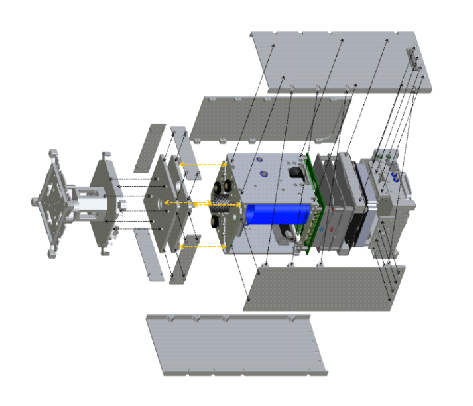
\includegraphics[width=0.6\textwidth]{02/fig/2-3-2.eps}
	\caption{組み立て図}
	\label{2-3-2}
\end{figure}

図\ref{2-3-4}に本衛星の通信回線を示す.本衛星はコマンドアップリンクにアマチュアVHF帯,テレメトリダウンリンクにアマチュアUHF帯を用いる.アンテナはいずれも展開式の半波長モノポールアンテナ(特注品のリン青銅製コンベックステープ)を使用する.地上局については既存の東工大局のハードウェアおよびソフトウェアを一部更新して用いた.
さらに,5.84GHz通信を実現するため,FITSAT-1で用いたものと同等の通信機(ロジカルプロダクト社LPTX5840-1,出力2W)を衛星に搭載する.衛星に搭載した5.84GHz円偏波パッチアンテナは購入品では性能が低かったため新規開発し搭載した.地上局については,FITSAT-1で用いたのと同等のLNB (Low Noise Block Converter)を購入し,東京工業大学が保有していたパラボラアンテナに設置した.これにより,アマチュア5.8GHz帯で最大115kbpsの通信を行う.パッチアンテナはバス部の端面に取り付けられる.本アンテナは半値幅約60 degの指向性であり,これを地上へ向ける姿勢制御が必要である.本衛星では,FITSAT-1にて実績のある,永久磁石を用いた沿磁力線姿勢制御を行う.角速度のダンピングについては,PCパーマロイの板を用いたヒステリシスダンパにより行う.姿勢制御の概要を図\ref{2-3-5}に示す.
\begin{figure}[H]
	\centering
	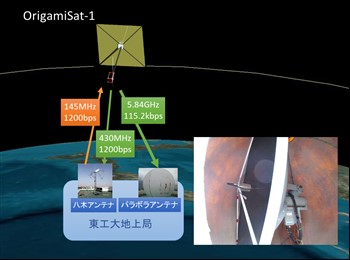
\includegraphics[width=0.6\textwidth]{02/fig/2-3-4.jpg}
	\caption{通信回線の概要}
	\label{2-3-4}
\end{figure}
\begin{figure}[H]
	\centering
	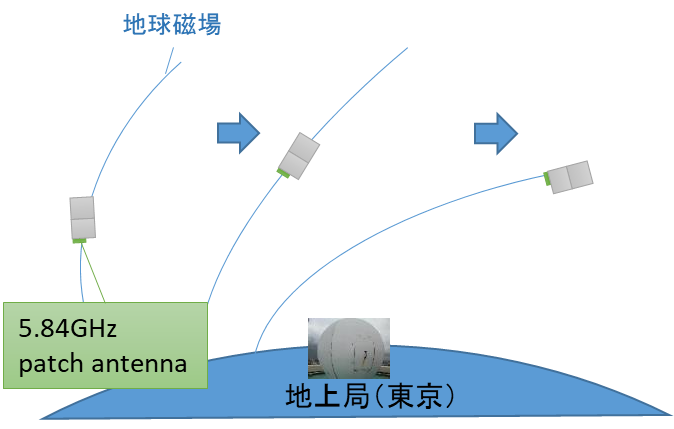
\includegraphics[width=0.5\textwidth]{02/fig/2-3-5.png}
	\caption{永久磁石を用いた沿磁力線制御}
	\label{2-3-5}
\end{figure}

\subsection{システムダイアグラム}
OrigamiSat-1 のシステムダイアグラムを図\ref{2-3-3}に示す.
\begin{figure}[H]
	\centering
	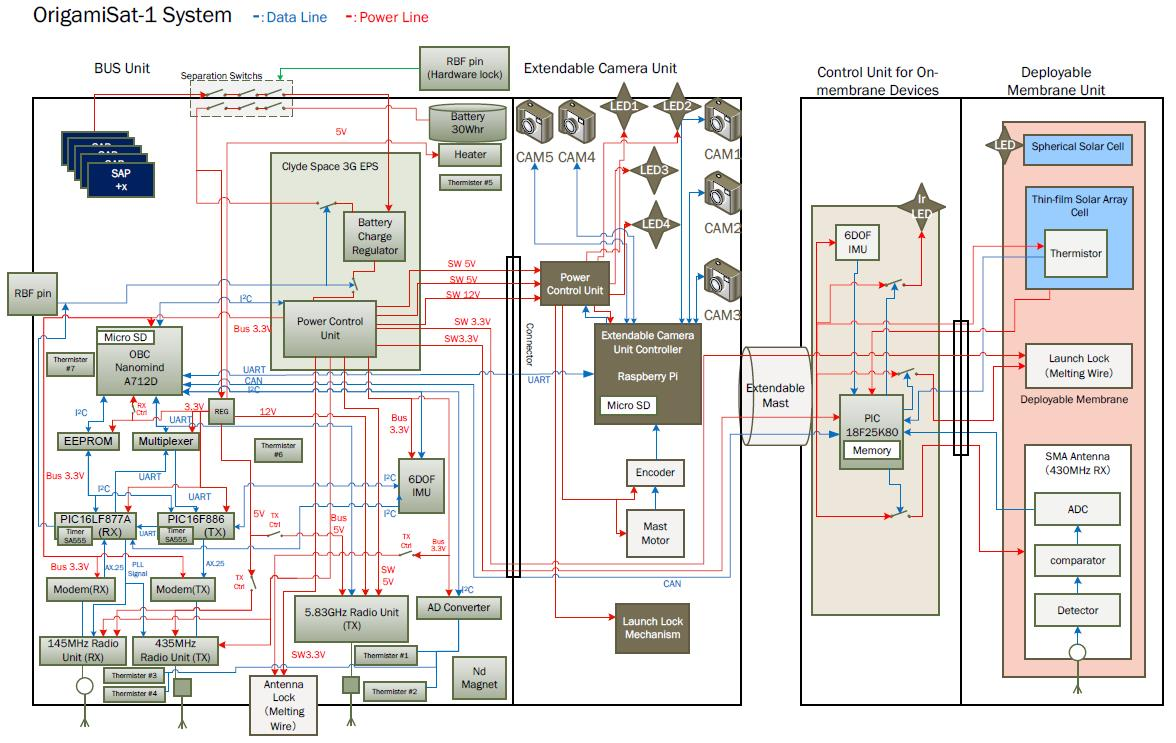
\includegraphics[width=1.0\textwidth]{02/fig/2-3-3.jpg}
	\caption{OrigamiSat-1フライトモデルのシステムダイアグラム}
	\label{2-3-3}
\end{figure}